\documentclass[a4paper,12pt]{article}
\usepackage{fullpage, float, graphicx}
\title{CS26410 Report 1\\
Simulation and Occupancy Grids}
\author{Chris Savill\\\texttt{chs17@aber.ac.uk}}
\begin{document}
\maketitle
\newpage
\tableofcontents
\newpage

\section{Player}
\noindent \textbf{Player} is an open source robot interface tool that takes code and translates that code into instructions for a robot. Player communicates with the hardware of a robot and such as a sonar sensor or the motors and allows you to use your code to control them as well as receiving any information that can be given back to the code vice versa. In technical terms, Player is a \textbf{Hardware/Robot Abstraction Layer}, or in simple terms, a middleman between the code and robot hardware.

\vspace{5mm}
\noindent Player supports a wide variety of devices and robot platforms, used widely in robotics research. Player is also widely used not only because it is part of an open source project for robotics research but because of the number of programming languages and operating systems it supports.

\section{Stage}
\textbf{Stage} is a 2D robot simulation tool that when used with Player (known as Player/Stage) provides a simulated environment to test your robot' code. Gazebo is the 3D simulation version of Stage. Able to simulate multiple robots concurrently, Stage is an excellent robot simulation tool.

\vspace{5mm}
\noindent Stage is able to interface with Player thus being able simulate a robot in a simulated world. Player would take your code and gives it to Stage which would then simulate the robot taking the translated instructions and acting accordingly. Also Stage is able to give information back to Player such as sonar readings, robot coordinates etc for Player to use with the code. Of course Player would have to request this information from Stage, but this is done in the exact same way as interfacing with a real robot's hardware. This is why Player and Stage are great for robotics research; the code you give to Player works with both a real robot (one supported) and Stage without much changes being made at all.

\section{Developing Robots with Player and Stage}
\noindent Player and Stage combined together provide a good and easy way of developing and testing code for robots. One main advantage of using Player/Stage is that you don't actually need a real robot, you can just test your code on a simulated robot in a virtual environment. This also preferred as your code may cause a real robot to become damaged in some way as well as drain power.

\vspace{5mm}
\noindent Another advantage of Player/Stage is that Stage allows you to have multiple robots in one simulation thus adding to the power of the platform for developing and testing purposes. One thing to mention is that although simulations can be good for developing and testing robots, the simulations tend to emulate an ideal environment where the real world is full on uncertainties. So to get better and more accurate results, all of the features of the real environment should be taken into account when building a simulated world for the robots. Also the simulations of the robots tend to emulate that of robots in top condition with no faults. So that must be taken into account when developing and testing your robots.

\section{Solution to Problem}

\subsection{Problem}
\noindent The problem to be solved is to engineer a way to map out an 'occupancy grid' of an area/environment given through a technique called \textbf{Occupancy Grid Mapping}. The purpose of an occupancy grid is to represent an environment as a grid of evenly sized cells where each cell is either marked as \textbf{full} or \textbf{empty} depending on whether there is an obstacle present in the location the cell \textit{overlays}.

\vspace{5mm}
\noindent One certain constraint of the problem is that the sizes of the cells must be 60cm by 60cm. The main issues I thought about were:

\begin{itemize}
	\item How to make the robot move a certain distance in a specified direction.
	\item How to control the exploration of the robot, should the robot explore in a spiral manner or a random search.
	\item Which sonar sensors on the sonar array to utilise to map out the occupancy grid.
	\item How to actually map out the occupancy grid with relation to the robot's environment.
\end{itemize}
 
\subsection{Solution}
\noindent My initial approach to solving the problem involved tackling each of the issues mentioned in the subsection above one at a time. However, as I eventually noticed that all of the issues are interlinked in one way or another so I had to accept that my designs may change as I try to get everything to integrate well together.

\vspace{5mm}
\noindent I first decided on how to construct an actual occupancy grid to map with. The specification stated that a 2D array of integers would be a good starting point. I though about how the occupancy grid would be used and if simple integer cells within the 2D array would suffice. This led me to think about how I would control the robot's exploration of an area.

\vspace{5mm}
\noindent After thinking of ways to tackle the exploration issue, I decided that obstacles would cause a problem with a random and fixed search and that a method of manoeuvring around the obstacles (if possible) would be required. When looked from a different perspective, the exploration problem looked like a search problem with the problem space being the exploration area in question. An artificial intelligence inspired search technique called Depth-First Search (DFS) was then chosen to control the robot's exploration.

\vspace{5mm}
\noindent The main idea with using DFS is that a stack(last in, first out) data structure would be used to store the path the robot has travelled along. The algorithm for managing the \textbf{path stack} is shown below:

\begin{itemize}
	\item Mark the current cell the robot currently occupies at explored.
	\item If the cell has neighbours left to explore, the direction to travel in next is randomised between those cells left to explore. The direction the robot then leaves in is added to the top of the path stack.
	\item If the current cell has no more neighbour cells left to explore, the robot will travel in the direction it just came from by using the direction stored at the top of the path stack and also popping it off.
\end{itemize}

\begin{figure}[H]
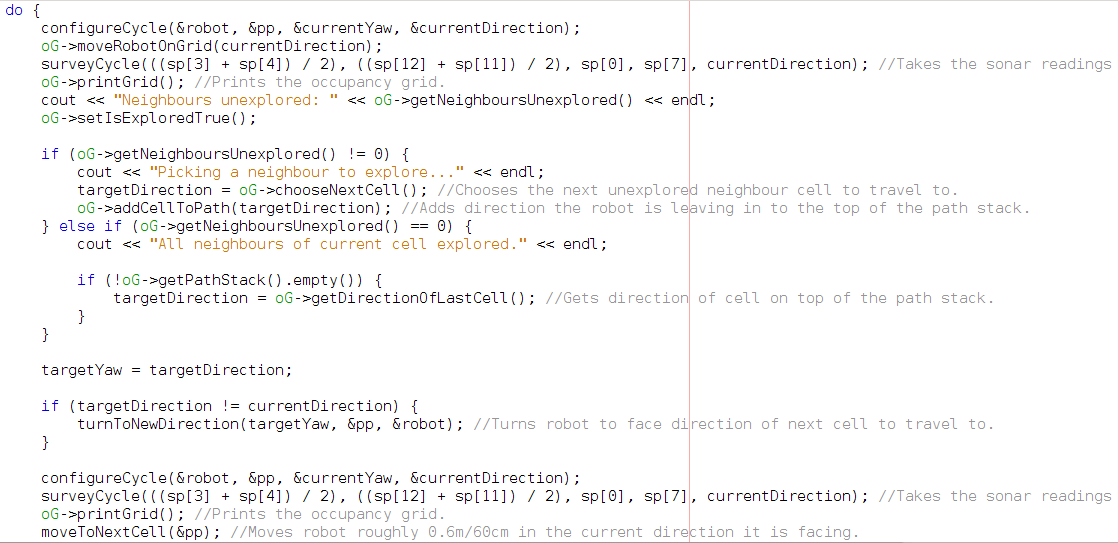
\includegraphics[scale=0.53]{robotics3DFS.png}
\caption{Screen shot of the DFS exploration algorithm implemented in C++.}
\end{figure}

\vspace{5mm}
\noindent As the path is stored as a stack the search acts like a Depth-First Search always going further and further until it hits a dead-end and then back tracks one cell, and tries again, and so fourth etc. This allows the robot to explore an entire area and even get around obstacles as it doesn't need to think about how it is going to get around it, the robot just eventually check every cell it can as that is how the search algorithm works.

\vspace{5mm}
\noindent Once I knew how the exploration would be controlled I knew what would be needed to keep track of the search and this led to 2D array of \textbf{Cell} structs which store not only the obstacle value, but other fields required for search purposes as well. Concerning the issue of which sonar sensors to use, it seemed sensible to only use the front, rear, left and right sonar sensors as they would be more accurate and easier to work with. This did meant that the robot would only be able to scan in directions at 90 degrees (approximately). Also for simplicity and to reduce error probabilities and effects, it made sense to only move one cell, that is 60cm approximately at a time in any 90 degree direction and only scan for obstacles 60cm approximately in either direction to map onto the grid, this occurred when deciding to use a DFS approach to exploration.

\vspace{5mm}
\noindent Also with those simplicities decided, it made to it easier to see how the 2D grid would lay over the robot's environment. A simple algorithm to consisting of \textbf{if statements} would move the robot on the grid with every move it made. And as the DFS approach allows for the robot to explore an area of undefined size, it occurred that the 2D grid would have to be dynamically resizeable so algorithms were implemented to resize the grid by 1 in the direction it just travelled. Algorithms to shift the values within the grid right and up were implemented as well for when the grid expands left and down to avoid using negative index values which would not work with arrays.

\subsection{Example Execution of Solution}

\begin{figure}[H]
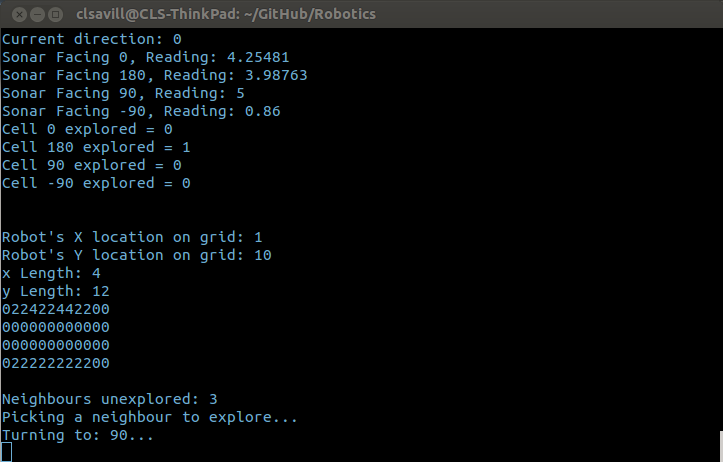
\includegraphics[scale=0.8]{robotics1Terminal.png}
\caption{Screen shot of the terminal window during an execution of the solution described above.}
\end{figure}

\begin{figure}[H]
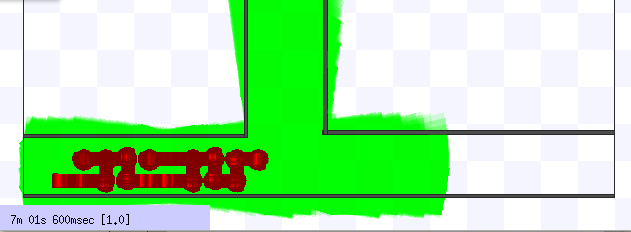
\includegraphics[scale=0.9]{robotics2Stage.png}
\caption{Screen shot of the Stage window during an execution of the solution described above.}
\end{figure}

\noindent The two screen shots above show an example execution of the solution implemented. Both the screen shots are of the same execution and time (cut from a full-screen screen shot), that is to say they are synchronised. The terminal window shows the state of the occupancy grid at the time the robot last scanned (scans every time it arrives at a cell and before it leaves). The Stage window shows the robots path. Take notice that the green painting is not at all a true representation of the robot's scans but the furthest any of it's sensors had managed to extend to.

\vspace{5mm}
\noindent The Stage window screen shot shows how the DFS algorithm can work, you can see back tracking in the robot's path and this also relates to the higher obstacle values on the terminal window screen shot. In terms of a threshold value needed to give a final view of the occupancy grid, taking a mean from all the cells that have an obstacle value > 0 would be appropriate although this value can change a lot if the robot does a lot of backtracking.

\end{document}